\section{Unmanned aerial vehicle}
\label{sec:unmanned-aerial-vehicle}
%
%
An unmanned aerial vehicle (UAV) (commonly known as a drone) is an aircraft 
without a human pilot on board and a type of unmanned vehicle. 
UAVs are a component of an unmanned aircraft system (UAS); which include a UAV,
a ground-based controller, and a system of communications between the two.\\  
The flight of UAVs may operate with various degrees of autonomy: either under
remote control by a human operator or autonomously by on-board computers.
Compared to crewed aircraft, UAVs were originally used for missions too
dangerous for humans.\cite{budiansky2005air}\\
While they originated mostly in military applications, their use is rapidly
expanding to commercial, scientific, recreational, agricultural, policing and
surveillance, product deliveries, aerial photography, infrastructure
inspections, and drone racing.\cite{wiki:uav}
%
%
\subsection{UAV components}
\label{ssec:components}
%
Crewed and un-crewed aircraft of the same type generally have recognizably
similar physical components.  One of difference are absence the cockpit and
environmental control system or life support systems.  
Some UAVs carry payloads such as a camera or other kinds sensors smaller and 
lightweight.
Small UAVs has assumed a characteristic quad-copter design particular
recognizable, although other scheme are realizable. 
Continuous development introduced new part or revisited thus the process of
miniaturized that require less-power propulsion and increase the battery
runtime.\\
Control systems for UAVs are different for remote human control, a camera
and video link almost always replace the cockpit windows; radio-transmitted
digital commands replace physical cockpit controls. Autopilot software is used
on both crewed and uncrewed aircraft, with varying feature sets.\cite{wiki:uav}
%
%
\begin{figure}[htb]
    \centering
    \subfloat[][\emph{typical quadcopter design}.\label{subfig:quadcopter-design}]{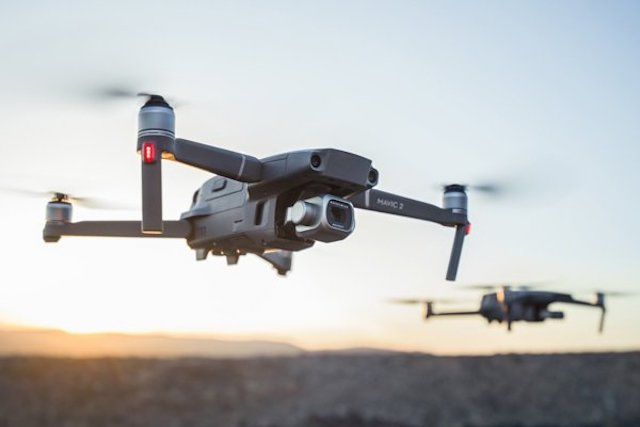
\includegraphics[width=.50\textwidth]{dji_mavic_2-1.jpg}} \\
    \subfloat[][\emph{multirotor drone design}.\label{subfig:multicopter}]{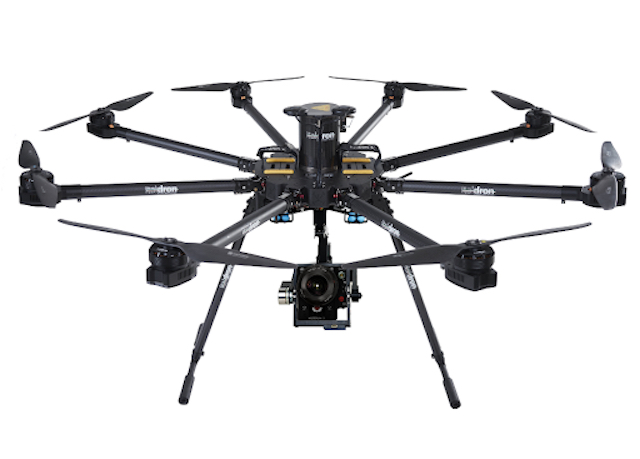
\includegraphics[width=.50\textwidth]{unnamed.jpg}} \\
    \captionsource{Example of design choices in the realization of UAVs shape}{
    \href{https://www.dji-store.it/guida-acquisto-migliori-droni-dji-per-riprese-aeree/}{DJI}; 
    \href{http://www.italdron.com/it/droni-professionali-e-accessori/droni-professionali/bigone-8hse-pro}{Italdron}}
    \label{fig:uav-design}
\end{figure}
%
%
\paragraph{Body} UAVs assume different configuration based on requirement of
task they perform for example aerial video shooting, surveys, territorial
control and many more.
Thus they are normally equipped with 4, 6, or 8 motor called quadcopter,
exacopter or octocopter.
The mainly difference that exist between different configuration is the payload
capacity that it can carry in flight.

\paragraph{Power supply}
Small UAVs mostly use lithium-polymer batteries (Li-Po), while larger vehicles
rely on conventional airplane engines. Scale or size of aircraft is not the
defining or limiting characteristic of energy supply for a UAV. 
Battery elimination circuitry (BEC) is used to centralize power distribution and
often harbors a microcontroller unit (MCU). Costlier switching BECs diminish
heating on the platform.\cite{wiki:uav}

% Computing[modifica]
% UAV computing capability followed the advances of computing technology, beginning with analog controls and evolving into microcontrollers, then system-on-a-chip (SOC) and single-board computers (SBC).

% System hardware for small UAVs is often called the flight controller (FC), flight controller board (FCB) or autopilot.

% Sensors[modifica]
% Position and movement sensors give information about the aircraft state. Exteroceptive sensors deal with external information like distance measurements, while exproprioceptive ones correlate internal and external states.[52]

% Non-cooperative sensors are able to detect targets autonomously so they are used for separation assurance and collision avoidance.[53]

% Degrees of freedom (DOF) refers to both the amount and quality of sensors on board: 6 DOF implies 3-axis gyroscopes and accelerometers (a typical inertial measurement unit – IMU), 9 DOF refers to an IMU plus a compass, 10 DOF adds a barometer and 11 DOF usually adds a GPS receiver.[54]

% Actuators[modifica]
% UAV actuators include digital electronic speed controllers (which control the RPM of the motors) linked to motors/engines and propellers, servomotors (for planes and helicopters mostly), weapons, payload actuators, LEDs and speakers.

% Software[modifica]
% UAV software called the flight stack or autopilot. UAVs are real-time systems that require rapid response to changing sensor data. Examples include Raspberry Pis, Beagleboards, etc. shielded with NavIO, PXFMini, etc. or designed from scratch such as Nuttx, preemptive-RT Linux, Xenomai, Orocos-Robot Operating System or DDS-ROS 2.0.

% Loop principles[modifica]

% Typical flight-control loops for a multirotor
% UAVs employ open-loop, closed-loop or hybrid control architectures.

% Open loop – This type provides a positive control signal (faster, slower, left, right, up, down) without incorporating feedback from sensor data.
% Closed loop – This type incorporates sensor feedback to adjust behavior (reduce speed to reflect tailwind, move to altitude 300 feet). The PID controller is common. Sometimes, feedforward is employed, transferring the need to close the loop further.[55]
% Flight controls[modifica]
% UAVs can be programmed to perform aggressive manœuvres or landing/perching on inclined surfaces,[56] and then to climb toward better communication spots.[57] Some UAVs can control flight with varying flight modelisation,[58][59] such as VTOL designs.

% UAVs can also implement perching on a flat vertical surface.[60]

% Communications[modifica]
% Most UAVs use a radio for remote control and exchange of video and other data. Early UAVs had only narrowband uplink. Downlinks came later. These bi-directional narrowband radio links carried command and control (C\& C) and telemetry data about the status of aircraft systems to the remote operator. For very long range flights, military UAVs also use satellite receivers as part of satellite navigation systems. In cases when video transmission was required, the UAVs will implement a separate analog video radio link.

% In the most modern UAV applications, video transmission is required. So instead of having 2 separate links for C\& C, telemetry and video traffic, a broadband link is used to carry all types of data on a single radio link. These broadband links can leverage quality of service techniques to optimize the C\& C traffic for low latency. Usually these broadband links carry TCP/IP traffic that can be routed over the Internet.

% The radio signal from the operator side can be issued from either:

% Ground control – a human operating a radio transmitter/receiver, a smartphone, a tablet, a computer, or the original meaning of a military ground control station (GCS). Recently control from wearable devices,[61] human movement recognition, human brain waves[62] was also demonstrated.
% Remote network system, such as satellite duplex data links for some military powers.[63] Downstream digital video over mobile networks has also entered consumer markets,[64] while direct UAV control uplink over the cellular mesh and LTE have been demonstrated and are in trials.[65]
% Another aircraft, serving as a relay or mobile control station – military manned-unmanned teaming (MUM-T).[66]
% A protocol MAVLink is increasingly becoming popular to carry command and control data between the ground control and the vehicle

\subsection{Autonomy}


% ICAO classifies uncrewed aircraft as either remotely piloted aircraft or fully autonomous.[67] Actual UAVs may offer intermediate degrees of autonomy. E.g., a vehicle that is remotely piloted in most contexts may have an autonomous return-to-base operation.

% Basic autonomy comes from proprioceptive sensors. Advanced autonomy calls for situational awareness, knowledge about the environment surrounding the aircraft from exterioceptive sensors: sensor fusion integrates information from multiple sensors.[52]

% Basic principles[modifica]
% One way to achieve autonomous control employs multiple control-loop layers, as in hierarchical control systems. As of 2016 the low-layer loops (i.e. for flight control) tick as fast as 32,000 times per second, while higher-level loops may cycle once per second. The principle is to decompose the aircraft's behavior into manageable "chunks", or states, with known transitions. Hierarchical control system types range from simple scripts to finite state machines, behavior trees and hierarchical task planners. The most common control mechanism used in these layers is the PID controller which can be used to achieve hover for a quadcopter by using data from the IMU to calculate precise inputs for the electronic speed controllers and motors.[citation needed]

% Examples of mid-layer algorithms:

% Path planning: determining an optimal path for vehicle to follow while meeting mission objectives and constraints, such as obstacles or fuel requirements
% Trajectory generation (motion planning): determining control maneuvers to take in order to follow a given path or to go from one location to another[68][69]
% Trajectory regulation: constraining a vehicle within some tolerance to a trajectory
% Evolved UAV hierarchical task planners use methods like state tree searches or genetic algorithms.[70]

% Autonomy features[modifica]

% UAV's degrees of autonomy
% UAV manufacturers often build in specific autonomous operations, such as:

% Self-level: attitude stabilization on the pitch and roll axes.
% Altitude hold: The aircraft maintains its altitude using barometric or ground sensors.
% Hover/position hold: Keep level pitch and roll, stable yaw heading and altitude while maintaining position using GNSS or inertal sensors.
% Headless mode: Pitch control relative to the position of the pilot rather than relative to the vehicle's axes.
% Care-free: automatic roll and yaw control while moving horizontally
% Take-off and landing (using a variety of aircraft or ground-based sensors and systems; see also:Autoland)
% Failsafe: automatic landing or return-to-home upon loss of control signal
% Return-to-home: Fly back to the point of takeoff (often gaining altitude first to avoid possible intervening obstructions such as trees or buildings).
% Follow-me: Maintain relative position to a moving pilot or other object using GNSS, image recognition or homing beacon.
% GPS waypoint navigation: Using GNSS to navigate to an intermediate location on a travel path.
% Orbit around an object: Similar to Follow-me but continuously circle a target.
% Pre-programmed aerobatics (such as rolls and loops)